\begin{quote}
"`\textbf{Pastry} is a generic, scalable and efficient substrate for peer-to-peer 
applications. Pastry nodes form a decentralized, self-organizing and 
fault-tolerant overlay network within the Internet. Pastry provides efficient 
request routing, deterministic object location, and load balancing in an 
application-independent manner. Furthermore, Pastry provides mechanisms that 
support and facilitate application-specific object replication, caching, and 
fault recovery."'
\end{quote}

\section{Grundlagen}
Jeder Knoten erhält eine eindeutige 128 bit Adresse (NodeID).
Dies geschieht entweder zufällig, oder durch eine Verschlüsselungsfunktion, die
auf die IP Adresse angewendet wird. Die NodeID's bilden also einen Ring von
$0-2^{128}$ (vgl. \cite{Schindelhauer2004}).

\section{Struktur}
\label{struktur}
Pastry verwaltet drei unterschiedliche Informations-Mengen. Das
sind: 
\begin{itemize}
  \item Routing Tabelle
  \item Leaf Set
  \item Neighbourhood Set
\end{itemize}
In der Routing Tabelle sind Einträge der Art NodeID $\rightarrow$ (IP)Adresse
vorhanden. 
\begin{quote}
''Jeder Peer kennt für jeden Präfix $p$ der NodeID über dem Alphabet
$2^b$ und für jeden Buchstaben $x \epsilon \{0, . . . , 2^{b - 1}\}$ einen
Repräsentanten der mit $px$ anfängt''\cite{Schindelhauer2004}. 
\end{quote}  
Ist beispielsweise $b=2$ und $2^b=4$, werden also $2^{2}-1 = 3$ Einträge für
jeden Präfix des Knotens gespeichert (siehe Abb. \ref{pastryPointer}).
\newline Das Leaf
Set enthält NodeIDs numerisch naheliegender Knoten, also
den benachbarten Knoten gemäß der Anordnung auf dem Ring. Ist $l$ die Größe des
Leaf Sets, werden $l/2$ linke Nachbarn und $l/2$ rechte Nachbarn gespeichert
\cite{Schindelhauer2004}(siehe Abb. \ref{pastryPointer}). Beim
Einfügen neuer Knoten wird das Leaf Set stets aktualisiert. 

\begin{figure}[H]
  \centering 
  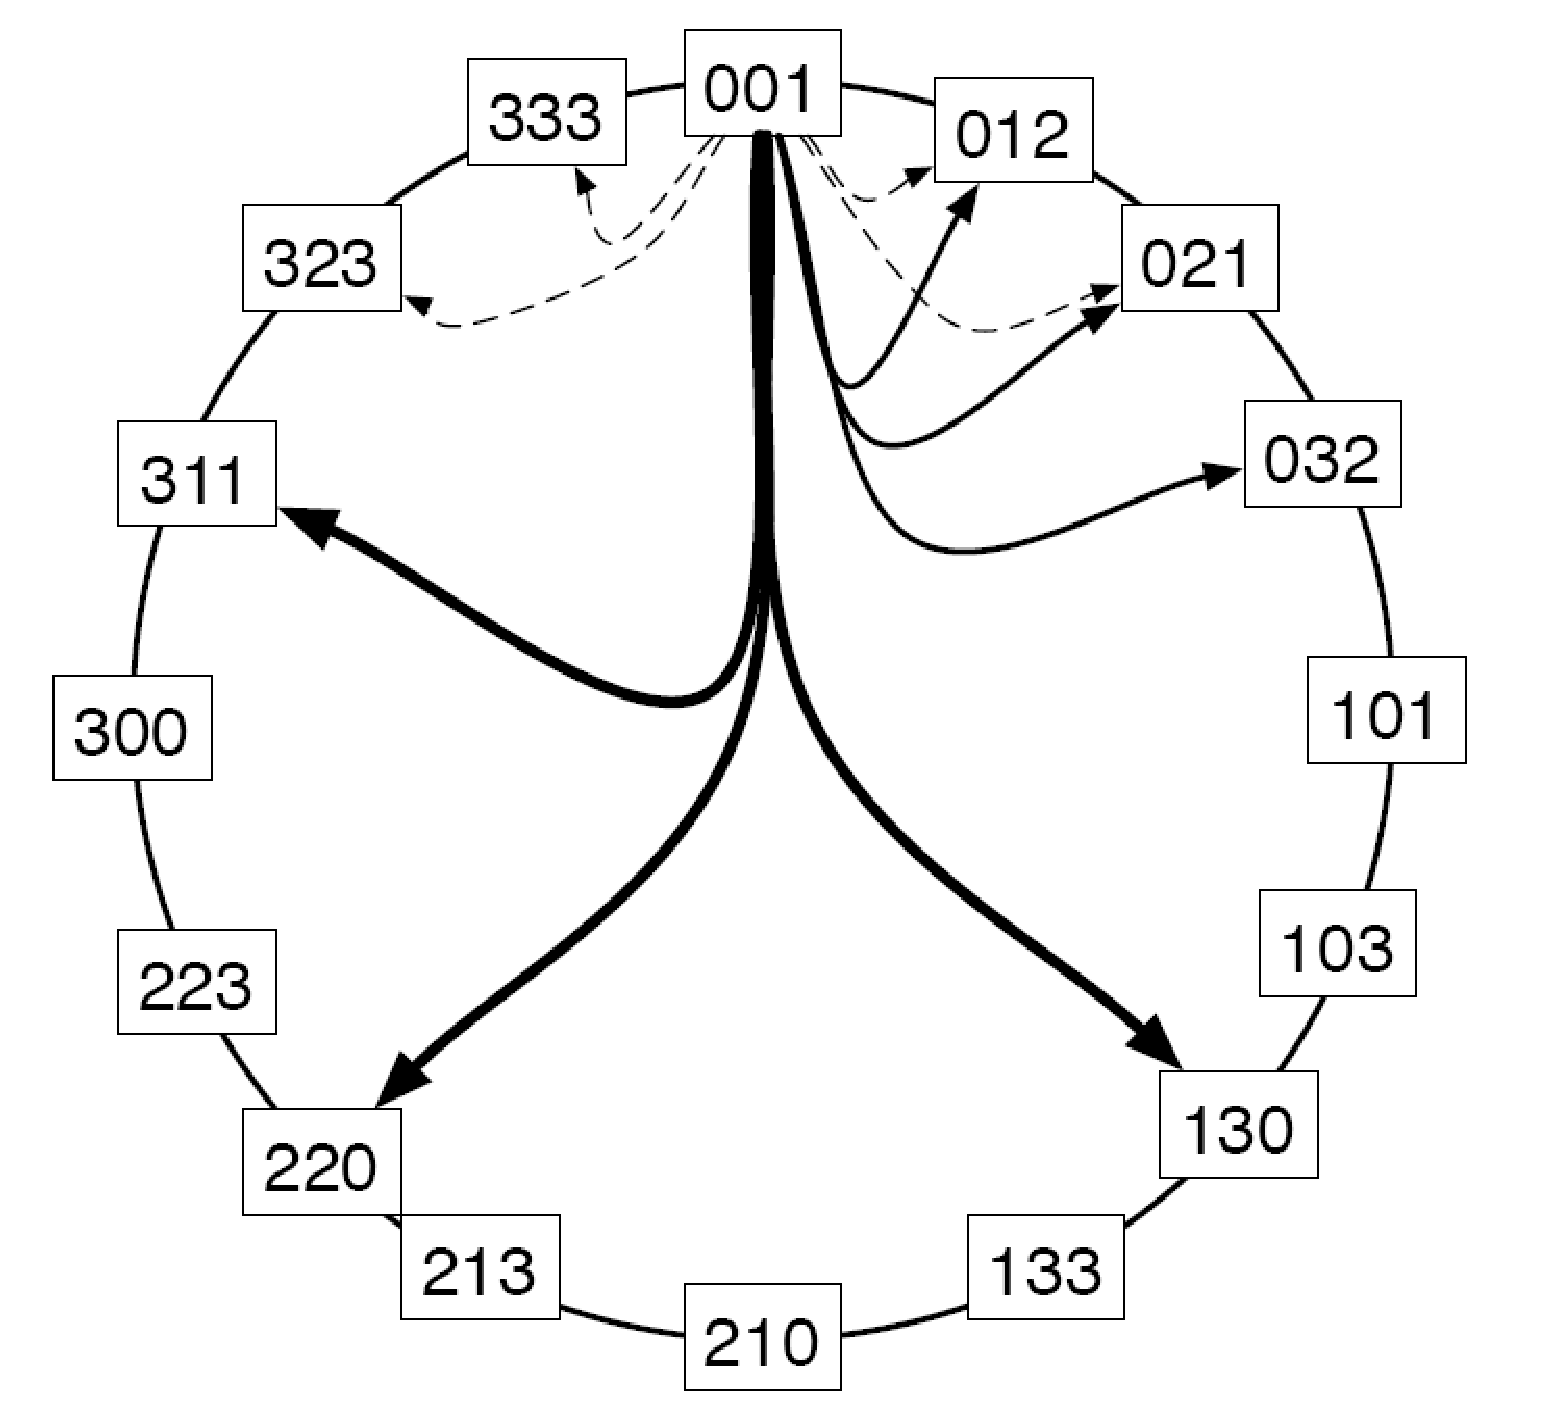
\includegraphics[width=0.5\textwidth]{../images/pastryPointer}
  \caption[Pastry Pointer]{Leaf Set(gestrichelt) und Routing Tabelle
  (durchgezogen) des Knotens $001$ für $b=2$ und $l=4$ \cite{Schindelhauer2004}}
  \label{pastryPointer}
\end{figure}
Im Neighbourhood Set werden Knoten gehalten, die
netzwerk-topologisch naheliegen. Dies wird durch heuristische Ansätze wie
PING-Zeit etc. realisiert.

\section{Routing}
Sollen nun Datenpakete weitergeleitet (geroutet) werden, macht man sich die im
vorangegangen Kapitel \ref{struktur} eingeführten Informationsmengen wie folgt
zunutze: 
\begin{enumerate}
  \item Durchsuche das Leaf Set nach dem Zielknoten. Ist er enthalten, wird das
  Paket dorthin weitergeleitet.
  \item Ansonsten wird die übereinstimmende Präfixlänge bestimmt, um das Paket
  anschließend an einen Knoten zu senden, dessen Präfix mindestens in einer
  Stelle mehr mit dem Zielknoten übereinstimmt.
  \item Schlägt dies ebenfalls fehl, werden alle 3 Komponenten auf den numerisch
  naheliegendsten Knoten durchsucht, an den das Paket dann schließlich
  weitergeleitet wird.
\end{enumerate}

\section{Organisation}
\subsection{Einfügen eines Knotens}
Zu Beginn sendet der Knoten, der in das bestehende Netzwerk eintreten möchte,
einen Request an einen beliebigen Knoten, der bereits in das Netzwerk
intergriert ist und fragt nach dessen Routingtabelle (vgl. Kapitel \ref{struktur})
Anschließend prüft er, wieviele Stellen der NodeID mit seiner eigenen
übereinstimmen und übernimmt genau so viele Zeilen aus der Routingtabelle.
Der angefragte Knoten informiert den zum neuen Knoten naheliegendsten Knoten
mit einer Nachricht. Jeder Zwischenknoten der die Nachricht
erhält sendet ebenfalls eine Nachricht an den neuen Knoten. So kann dieser seine
Routingtabelle vollständig ausfüllen. Der Empfängerknoten der Nachricht sendet
abschließend sein Leaf Set (vgl. Kapitel \ref{struktur}), welches der
neue Knoten übernimmt. 
Das Neighbourhood Set (vgl. Kapitel \ref{struktur}) übernimmt der neue
Knoten von dem initial gefragten Knoten. Dieses muss der neue Knoten
anschließend sukzessive verbessern, da ihm die topologische Entfernung des
initial gefragten Knotens natürlich nicht bekannt ist. (Vgl. \cite{Pastry})
Abbildung \ref{fig:pastry-insert-node} zeigt den Ablauf beim Einfügen des
Knotens mit der ID \texttt{1234}.

\begin{figure}[H]
  \centering 
  \def\JPicScale{0.70}
  %%Created by jPicEdt 1.4.1: mixed JPIC-XML/LaTeX format
%%Sun Jun 17 18:03:29 CEST 2007
%%Begin JPIC-XML
%<?xml version="1.0" standalone="yes"?>
%<jpic x-min="0.26" x-max="198.16" y-min="-1.3" y-max="114.21" auto-bounding="true">
%<g>
%<g>
%<ellipse fill-color= "#999999"
%	 shadow-color= "#666666"
%	 p3= "(40.26,33.16)"
%	 p2= "(40.26,53.16)"
%	 p1= "(0.26,53.16)"
%	 fill-style= "solid"
%	 closure= "open"
%	 angle-end= "0"
%	 shadow= "true"
%	 angle-start= "0"
%	 />
%<text text-vert-align= "center-v"
%	 fill-style= "none"
%	 anchor-point= "(20.26,43.16)"
%	 text-frame= "noframe"
%	 text-hor-align= "center-h"
%	 >
%1234
%</text>
%</g>
%<g>
%<ellipse fill-color= "#cccccc"
%	 shadow-color= "#666666"
%	 p3= "(115.26,33.16)"
%	 p2= "(115.26,53.16)"
%	 p1= "(75.26,53.16)"
%	 fill-style= "solid"
%	 closure= "open"
%	 angle-end= "0"
%	 shadow= "true"
%	 angle-start= "0"
%	 />
%<text text-vert-align= "center-v"
%	 fill-style= "none"
%	 anchor-point= "(95.26,43.16)"
%	 text-frame= "noframe"
%	 text-hor-align= "center-h"
%	 >
%5678
%</text>
%</g>
%<g>
%<ellipse fill-color= "#cccccc"
%	 shadow-color= "#666666"
%	 p3= "(195.26,78.16)"
%	 p2= "(195.26,98.16)"
%	 p1= "(155.26,98.16)"
%	 fill-style= "solid"
%	 closure= "open"
%	 angle-end= "0"
%	 shadow= "true"
%	 angle-start= "0"
%	 />
%<text text-vert-align= "center-v"
%	 fill-style= "none"
%	 anchor-point= "(175.26,88.16)"
%	 text-frame= "noframe"
%	 text-hor-align= "center-h"
%	 >
%1238
%</text>
%</g>
%<g>
%<ellipse fill-color= "#cccccc"
%	 shadow-color= "#666666"
%	 p3= "(135.26,63.16)"
%	 p2= "(135.26,83.16)"
%	 p1= "(95.26,83.16)"
%	 fill-style= "solid"
%	 closure= "open"
%	 angle-end= "0"
%	 shadow= "true"
%	 angle-start= "0"
%	 />
%<text text-vert-align= "center-v"
%	 fill-style= "none"
%	 anchor-point= "(115.26,73.16)"
%	 text-frame= "noframe"
%	 text-hor-align= "center-h"
%	 >
%1352
%</text>
%</g>
%<g>
%<ellipse fill-color= "#cccccc"
%	 shadow-color= "#666666"
%	 p3= "(185.26,33.16)"
%	 p2= "(185.26,53.16)"
%	 p1= "(145.26,53.16)"
%	 fill-style= "solid"
%	 closure= "open"
%	 angle-end= "0"
%	 shadow= "true"
%	 angle-start= "0"
%	 />
%<text text-vert-align= "center-v"
%	 fill-style= "none"
%	 anchor-point= "(165.26,43.16)"
%	 text-frame= "noframe"
%	 text-hor-align= "center-h"
%	 >
%1263
%</text>
%</g>
%<multicurve stroke-style= "dashed"
%	 left-arrow= "head"
%	 fill-style= "none"
%	 stroke-dasharray= "1;1"
%	 points= "(75.26,43.16);(75.26,43.16);(40.26,43.16);(40.26,43.16)"
%	 />
%<text text-vert-align= "center-v"
%	 fill-style= "none"
%	 anchor-point= "(57.63,47.04)"
%	 text-frame= "noframe"
%	 text-hor-align= "center-h"
%	 >
%Join-Request
%</text>
%<text text-vert-align= "center-v"
%	 fill-style= "none"
%	 anchor-point= "(81.51,95.26)"
%	 text-frame= "noframe"
%	 text-hor-align= "center-h"
%	 >
%Routing-Tabelle
%</text>
%<text text-vert-align= "center-v"
%	 fill-style= "none"
%	 anchor-point= "(51.32,21.97)"
%	 text-frame= "noframe"
%	 text-hor-align= "center-h"
%	 >
%Neighborhood-Set u.
%</text>
%<text text-vert-align= "center-v"
%	 fill-style= "none"
%	 anchor-point= "(103.95,114.21)"
%	 text-frame= "noframe"
%	 text-hor-align= "center-h"
%	 >
%Leaft-Set + Routing-Tabelle
%</text>
%<multicurve stroke-width= "0.5"
%	 left-arrow= "head"
%	 fill-style= "none"
%	 points= "(103.42,64.93);(103.42,64.93);(96.32,53.36);(96.32,53.36)"
%	 />
%<multicurve left-arrow= "head"
%	 fill-style= "none"
%	 points= "(100.99,18.09);(100.99,18.09);(95.99,33.09);(95.99,33.09)"
%	 />
%<multicurve stroke-width= "0.5"
%	 left-arrow= "head"
%	 fill-style= "none"
%	 points= "(149.87,49.67);(149.87,49.67);(131.97,67.57);(131.97,67.57)"
%	 />
%<multicurve left-arrow= "head"
%	 fill-style= "none"
%	 points= "(115.26,83.16);(115.26,83.16);(110.26,98.16);(110.26,98.16)"
%	 />
%<multicurve stroke-width= "0.5"
%	 left-arrow= "head"
%	 fill-style= "none"
%	 points= "(172.24,78.22);(172.24,78.22);(167.89,53.22);(167.89,53.22)"
%	 />
%<multicurve left-arrow= "head"
%	 fill-style= "none"
%	 points= "(198.16,57.63);(198.16,57.63);(183.16,47.63);(183.16,47.63)"
%	 />
%<pscurve stroke-width= "0.5"
%	 stroke-color= "#ff0000"
%	 fill-style= "none"
%	 right-arrow= "head"
%	 closed= "false"
%	 curvature= "1;0.1;0"
%	 points= "(169.74,90.53);(167.37,92.89);(116.05,110.79);(62.89,105.53);(30,79.74);(20.26,50);
%	(19.21,43.42)"
%	 />
%<pscurve stroke-width= "0.5"
%	 stroke-color= "#ff0000"
%	 fill-style= "none"
%	 right-arrow= "head"
%	 closed= "false"
%	 curvature= "1;0.1;0"
%	 points= "(91.18,40.86);(90.99,37.11);(80,23.68);(51.25,18.49);(25.13,23.88);(19.8,36.64);
%	(20.72,39.14)"
%	 />
%<pscurve stroke-width= "0.5"
%	 stroke-color= "#ff0000"
%	 fill-style= "none"
%	 right-arrow= "head"
%	 closed= "false"
%	 curvature= "1;0.1;0"
%	 points= "(113.95,75.53);(112.11,79.21);(93.95,91.32);(58.62,87.63);(40.79,72.37);(26.05,49.21);
%	(24.47,45)"
%	 />
%<pscurve stroke-width= "0.5"
%	 stroke-color= "#ff0000"
%	 fill-style= "none"
%	 right-arrow= "head"
%	 closed= "false"
%	 curvature= "1;0.1;0"
%	 points= "(158.75,42.17);(166.32,36.58);(144.61,10.13);(96.05,2.11);(13.42,18.95);(8.95,41.32);
%	(11.05,42.11)"
%	 />
%<text text-vert-align= "center-v"
%	 fill-style= "none"
%	 anchor-point= "(90.79,5.53)"
%	 text-frame= "noframe"
%	 text-hor-align= "center-h"
%	 >
%Routing-Tabelle
%</text>
%<text text-vert-align= "center-v"
%	 fill-style= "none"
%	 anchor-point= "(50.46,15.13)"
%	 text-frame= "noframe"
%	 text-hor-align= "center-h"
%	 >
%Routing-Tabelle
%</text>
%</g>
%</jpic>
%%End JPIC-XML
%PSTricks content-type (pstricks.sty package needed)
%Add \usepackage{pstricks} in the preamble of your LaTeX file
%You can rescale the whole picture (to 80% for instance) by using the command \def\JPicScale{0.8}
\ifx\JPicScale\undefined\def\JPicScale{1}\fi
\psset{unit=\JPicScale mm}
\psset{linewidth=0.3,dotsep=1,hatchwidth=0.3,hatchsep=1.5,shadowsize=1,dimen=middle}
\psset{dotsize=0.7 2.5,dotscale=1 1,fillcolor=black}
\psset{arrowsize=1 2,arrowlength=1,arrowinset=0.25,tbarsize=0.7 5,bracketlength=0.15,rbracketlength=0.15}
\begin{pspicture}(0,0)(198.16,114.21)
\newrgbcolor{userFillColour}{0.6 0.6 0.6}
\newrgbcolor{userShadowColour}{0.4 0.4 0.4}
\rput{0}(20.26,43.16){\psellipse[fillcolor=userFillColour,fillstyle=solid,shadow=true,shadowcolor=userShadowColour](0,0)(20,-10)}
\rput(20.26,43.16){1234}
\newrgbcolor{userFillColour}{0.8 0.8 0.8}
\newrgbcolor{userShadowColour}{0.4 0.4 0.4}
\rput{0}(95.26,43.16){\psellipse[fillcolor=userFillColour,fillstyle=solid,shadow=true,shadowcolor=userShadowColour](0,0)(20,-10)}
\rput(95.26,43.16){5678}
\newrgbcolor{userFillColour}{0.8 0.8 0.8}
\newrgbcolor{userShadowColour}{0.4 0.4 0.4}
\rput{0}(175.26,88.16){\psellipse[fillcolor=userFillColour,fillstyle=solid,shadow=true,shadowcolor=userShadowColour](0,0)(20,-10)}
\rput(175.26,88.16){1238}
\newrgbcolor{userFillColour}{0.8 0.8 0.8}
\newrgbcolor{userShadowColour}{0.4 0.4 0.4}
\rput{0}(115.26,73.16){\psellipse[fillcolor=userFillColour,fillstyle=solid,shadow=true,shadowcolor=userShadowColour](0,0)(20,-10)}
\rput(115.26,73.16){1352}
\newrgbcolor{userFillColour}{0.8 0.8 0.8}
\newrgbcolor{userShadowColour}{0.4 0.4 0.4}
\rput{0}(165.26,43.16){\psellipse[fillcolor=userFillColour,fillstyle=solid,shadow=true,shadowcolor=userShadowColour](0,0)(20,-10)}
\rput(165.26,43.16){1263}
\psline[linestyle=dashed,dash=1 1]{<-}(75.26,43.16)(40.26,43.16)
\rput(57.63,47.04){{\tiny Join-Request}}
\rput(81.51,95.26){{\tiny Routing-Tabelle}}
\rput(51.32,21.97){{\tiny Neighborhood-Set u.}}
\rput(103.95,114.21){{\tiny Leaft-Set + Routing-Tabelle}}
\psline[linewidth=0.5]{<-}(103.42,64.93)(96.32,53.36)
\psline{<-}(100.99,18.09)(95.99,33.09)
\psline[linewidth=0.5]{<-}(149.87,49.67)(131.97,67.57)
\psline{<-}(115.26,83.16)(110.26,98.16)
\psline[linewidth=0.5]{<-}(172.24,78.22)(167.89,53.22)
\psline{<-}(198.16,57.63)(183.16,47.63)
\psecurve[linewidth=0.5,linecolor=red,curvature=1.0 0.1 0.0]{->}(169.74,90.53)(167.37,92.89)(116.05,110.79)(62.89,105.53)(30,79.74)(20.26,50)(19.21,43.42)
\psecurve[linewidth=0.5,linecolor=red,curvature=1.0 0.1 0.0]{->}(91.18,40.86)(90.99,37.11)(80,23.68)(51.25,18.49)(25.13,23.88)(19.8,36.64)(20.72,39.14)
\psecurve[linewidth=0.5,linecolor=red,curvature=1.0 0.1 0.0]{->}(113.95,75.53)(112.11,79.21)(93.95,91.32)(58.62,87.63)(40.79,72.37)(26.05,49.21)(24.47,45)
\psecurve[linewidth=0.5,linecolor=red,curvature=1.0 0.1 0.0]{->}(158.75,42.17)(166.32,36.58)(144.61,10.13)(96.05,2.11)(13.42,18.95)(8.95,41.32)(11.05,42.11)
\rput(90.79,5.53){{\tiny Routing-Tabelle}}
\rput(50.46,15.13){{\tiny Routing-Tabelle}}
\end{pspicture}

  \caption[Pastry: Knoten einfügen]{Einfügen des Pastry-Knotens \texttt{1234}.}
  \label{fig:pastry-insert-node}
\end{figure}

\subsection{Austritt eines Knotens}
Pastry unterscheidet nicht zwischen freiwilligem und unfreiwilligem Austreten 
eines Knotens aus dem Netzwerk. Hierbei wird der Ansatz verfolgt, dass eine
Fehlerbehandlung bei unfreiwilligem Austreten eines Knotens ohnehin unerlässlich
ist. Wird ein Knoten gewollt aus dem Netzwerk entfernt, wird dies durch die
Fehlerbehandlungs-Routine mit übernommen. Diese Fehlerbehandlungs-Routine
muss 2 Fälle berücksichtigen:
\begin{enumerate}
  \item Tritt der Fehler im Leaf Set auf, schickt der Knoten einen Request an
  den Knoten, den er auf der gleichen Seite im Leaf Set hält, um dessen Leaf Set
  anzufordern. Anhand dessen ersetzt er den fehlerhaften Knoten in seinem Leaf
  Set durch einen neuen Knoten.
  \item Tritt der Fehler in der Routingtabelle auf, wird eine Nachricht an einen
  Knoten aus der Routingtabelle gesendet, der die gleiche Präfixübereinstimmung
  besitzt. Von diesem wird dann der Knoten angefordert, zu dem nicht geroutet
  werden konnte. Besitzt dieser den Zielknoten ebenfalls nicht, wird der nächste
  Knoten mit derselben Präfixübereinstimmung gefragt usw. Enthält kein Knoten
  mit diesem Präfix den Knoten, über den geroutet werden soll, wird die Suche
  um eine Ebene ausgedehnt, d. h. der Präfix wird verkürzt.  
\end{enumerate}
